% !TEX root = ./paper.tex
\label{sec:content}

This section describes several of the possible benefits of \tcpls
compared to keeping \tcp and \tls isolated.
We provide some use cases and experiment with the
connection application-level connection migration offered by our API. Other user
cases described in Section~\ref{sec:research} are flagged to the roadmap and we
expect them to further demonstrate the
strength of a more intertwined \tls/\tcp transport protocol.

Our current implementation offers:
%\begin{enumerate}[label=(\roman*)]
\textit{(i)} An experimental API that wraps \tls and \tcp and enables
    applications to
    handle multihoming, multipathing, and various transport layer mechanisms.
  \textit{(ii)} An improved \tcp extensibility mechanism that sends \tcp options
    through the secure \tcpls channel. We currently support the \tcp
    User Timeout option. Supporting another \tcp option is only a matter of
    extending the sender's API and processing the option
    on the receiver side. \tcpls's internal machinery can already send any \tcp
    option during or after the handshake.
\textit{(iii)} The ability for the server to send eBPF bytecode over the secure
  channel to upgrade the client's \tcp congestion control scheme or
  tune other \tcp mechanisms \cite{brakmo2017tcp, tran2019beyond}.
  \textit{(iv)} The support of parallel streams and multiplexing over \tcp connections
    with different cryptographic context.
%\end{enumerate}

\subsection{The \tcpls API}

The API that applications use to interact with a protocol plays an important
role in enabling them to leverage all the protocol features. The most
popular API to interact with the transport layer remains the BSD socket
API. Researchers and the IETF have explored new
ways to expose a transport API~\cite{draft-ietf-taps-arch,hruby2014sockets,rfc6458,hesmans2016enhanced,schmidt2013socket}.

In this spirit, application-level developers would only be required to
configure a \texttt{\tcpls} context and register function callbacks.
%We design \tcpls such
%that the application-level developers can ignore any notion of Network IPC as
%defined by, for example, the POSIX API, the Berkeley socket API or Winsock,
%facilitating application-level development by offering a more concrete
%session-level interface based on asynchronous network events.
%The overall idea is to offer to application developers the opportunity to tune
%the transport protocol for a better usage of the network from their own
%application protocol, which might depend on its distinguishing
%features.
%\todo{we need to explain the mpjoin}
To illustrate \tcpls API's flexibility, we consider a simple
use case inspired by Happy Eyeballs \cite{rfc8305}. This technique is
used by web browsers when interacting with dual-stack servers. They
try to establish \tcp connections using IPv4 and IPv6 and prefer the
one that offers the lowest latency. This avoids problems when an address
family is broken on a path but not the other and sometimes results in
lower latency \cite{bajpai2019longitudinal}.


\begin{figure}[t]
  \resizebox{0.49\textwidth}{!}{%
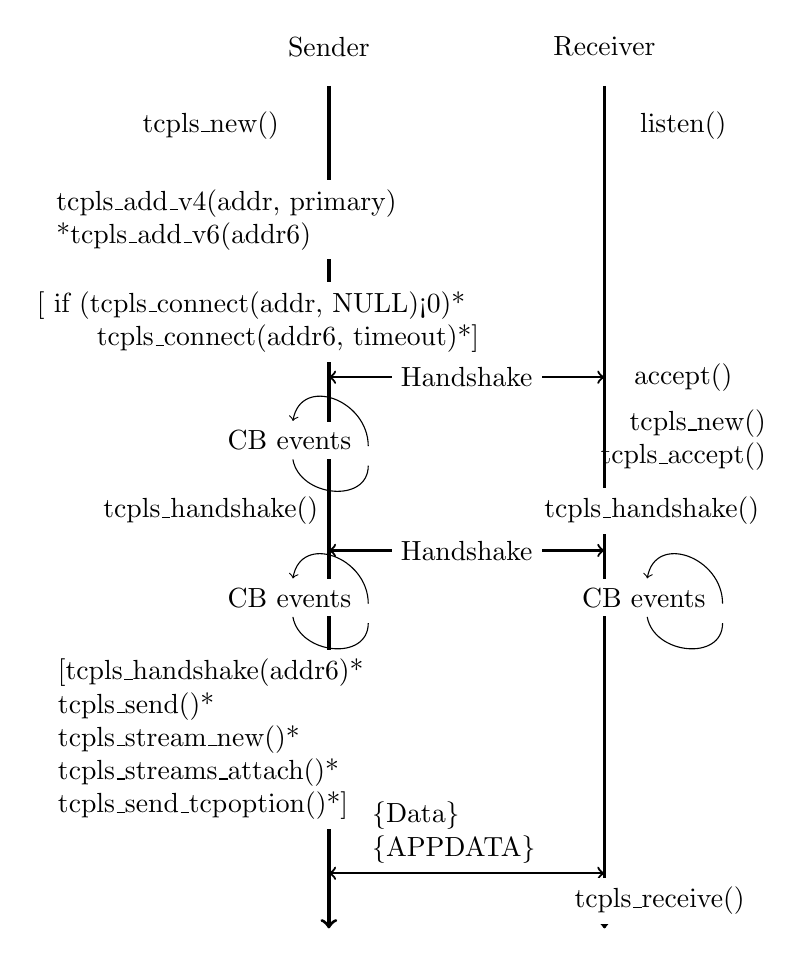
\begin{tikzpicture}
   \colorlet{lightgray}{black!20}
   \tikzstyle{arrow} = [thick,->,>=stealth]
   \tikzset{state/.style={rectangle, dashed, draw, fill=white} }
   \node[black, fill=white] at (0.5,10) {Sender};
   \node[black, fill=white] at (4,10) {Receiver};
   \draw[very thick,->] (0.5,9.5) -- (0.5,-1.2);
   \draw[very thick,->] (4,9.5) -- (4,-1.2);
   \node at (-1,9) {tcpls\_new()};
   \node at (5, 9) {listen()};
   \node[align=left, fill=white] at (-0.8,7.8) {tcpls\_add\_v4(addr,
     primary)\\*tcpls\_add\_v6(addr6)};
   \node[fill=white, align=left] at (-0.4,6.5) {[ if (tcpls\_connect(addr,
     NULL)<0)*\\
     \indent~~tcpls\_connect(addr6, timeout)*]};
   \draw[black, thick, <->] (0.5,5.8) -- (4,5.8) node [midway, fill=white] {\tcp Handshake};
   \node[fill=white] at (0,5) (Callback) {CB events};
   \node at (1,4.8) (here) {};
   \draw [->] (Callback) to[out=-80, in=-90,looseness=1.3] (here)
   to[out=90,in=80,looseness=1.5] (Callback);
   \node at (5, 5.8) {accept()};
   \node[align=right] at (5, 5) {tcpls\_new()\\tcpls\_accept()};
   \node at (-1,4.1) {tcpls\_handshake()};
   \node[fill=white] at (4.6,4.1) {tcpls\_handshake()};
   \draw[black, thick, <->] (0.5,3.6) -- (4,3.6) node [midway, fill=white] {\tcpls Handshake};
   \node[fill=white] at (0,3) (CB2) {CB events};
   \node at (1,2.8) (here2) {};
   \draw [->] (CB2) to[out=-80, in=-90,looseness=1.3] (here2)
   to[out=90,in=80,looseness=1.5] (CB2);
   \node[fill=white] at (4.5,3) (CB3) {CB events};
   \node at (5.5,2.8) (here3) {};
   \draw [->] (CB3) to[out=-80, in=-90,looseness=1.3] (here3)
   to[out=90,in=80,looseness=1.5] (CB3);
   \node[fill=white, align=left] at (-1, 1.2)
   {[tcpls\_handshake(addr6)*\\tcpls\_send()*\\tcpls\_stream\_new()*\\tcpls\_streams\_attach()*\\tcpls\_send\_tcpoption()*]};
   \draw[black, thick, <->] (0.5,-0.5) -- (4,-0.5) node [midway, fill=white,
   above, text width=2.4cm]
   {\{\tcpls Data\} \{APPDATA\}};
   \node[fill=white] at (4.7,-0.85) {tcpls\_receive()};
\end{tikzpicture}
}
\caption{API Workflow example. * means optional call, [ ] means optional call flow, and \{
  \} means encrypted.}
  \label{fig:api}
\end{figure}

Figure~\ref{fig:api}
shows an example of our current API workflow. The API can handle
explicit multipath techniques such as Happy Eyeball by chaining
\texttt{tcpls\_connect()} with an appropriate timeout of 50ms, as shown in the
Figure. \tcpls lets the application explicitly choose
the multipath mesh by calling several times \texttt{tcpls\_connect(src, dest,
  timeout)};. The application may configure callbacks to connection events that
would occur within \tcpls, such as a connection establishment, a stream
attachment, a multipath join, the reception of a \tcp option to tune TCP, and
more. When
multiple streams are attached to multiple \tcp connections, the application may
configure various \tcpls behaviours. Among them, we support HOL-blocking avoidance, aggregation of
bandwidth with multipathing, connection failover, and connection migration.
Note that, HOL-blocking avoidance is incompatible with the aggregation of bandwidth
with multipathing (the application can do either one but not both at the same
time).



%Note, those features are not stable yet, and many bugs remain to be fixed.

\subsection{On \tcp extensibility}
\label{sec:tcpoptions}

The \tcp specification limits the size of the entire \tcp header (including options)
to 64 bytes. Unfortunately, the \tcp designers did not foresee that so many \tcp
extensions would be standardized. Today, the size of the \tcp header
becomes a constraint. For example, it severely limits the number of gaps that
can be covered by selective acknowledgments. This gets worse with extensions
such as Multipath \tcp \cite{rfc6824} that consume more space in the \tcp header.
The IETF has discussed this problem for several years, but the latest attempt
to solve it \cite{draft-ietf-tcpm-tcp-edo-10} has not yet been implemented by
major \tcp stacks.

\tcpls provides more space for some \tcp options. First, with \tcpls, \tcp
options can be negotiated during the \tls handshake. Since the \tls messages are
included in the \tcp payload, there is more space to carry them. Another
advantage of this approach is that the TCP options are secured by \tls. This
implies that they cannot be modified by middleboxes. This could be an advantage,
but could also prevent \tcpls from correctly working through some types of
transparent TCP proxies.

Second, we can also carry \tcp options inside \tls records. For example, we used
this feature to implement the \tcp User Time Out option \cite{rfc5482}. A client
can use this option to set the maximum value of the retransmission
timer on a server. Linux \tcp has a socket option that allows setting
this timer locally, but it does not implement the option. With \tcpls, the client sends the option inside a \tls record, the server extracts it
and performs the required \texttt{setsockopt}.

\subsection{Multipathing}

\subsubsection{Application-level Connection Migration}
\label{sec:connmigr}

Given the availability of multiple IP paths, connection migration might be a
powerful tool to improve the application connection's reliability.  We
implement Connection migration and Failover as two distinct measures to handle
two different inquiries: 1) The application expects to take advantage of multiple
IP paths. 2) The application expects to be resilient to a network outage. In the
first case, we implement connection migration and multipathing from a
protocol viewpoint, as the same exchange of messages and API calls from \tcpls.
It is left for the application to decide and program
through the API calls whether it wants to move all the traffic from one path to
another or split the traffic among the available paths according to any
scheduling policy. The second
inquiry focuses on simply configuring \tcpls to automatically move the traffic to
another available IP-level path if a network outage is detected.
%The current implementation supports surviving abrupt reset of the connection,
%yet we may also want to
%monitor the connection and switch to another one if the path quality is low.


\subsubsection{Failover}
describing Failover

\subsubsection{Data Aggregation}
Describing orderings and schedulers

\subsection{0-RTT Connections}

